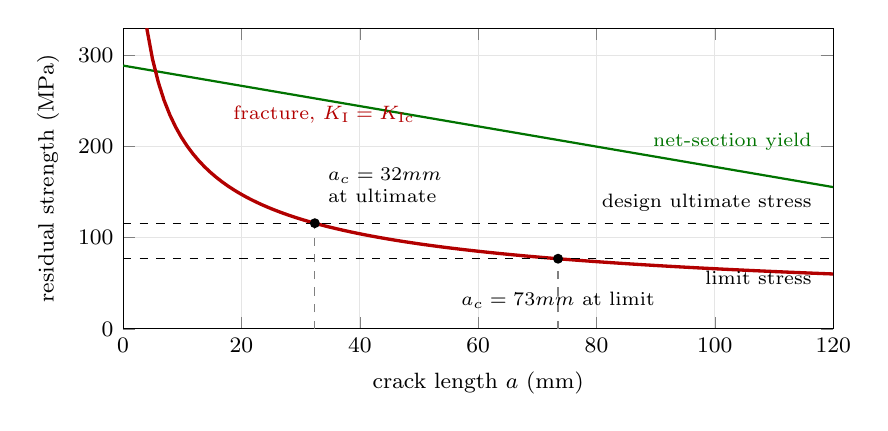
\begin{tikzpicture}
\begin{axis}[width=10.6cm,height=5.4cm,xlabel={crack length $a$ (mm)},ylabel={residual strength (MPa)},
 xmin=0,xmax=120,ymin=0,ymax=330,grid=both,grid style={gray!20},
 label style={font=\footnotesize},tick label style={font=\footnotesize}]
% net section yield line
\addplot[thick,green!45!black,domain=0:120,samples=2]{289*(1-x/260)};
% fracture line K=Kic
\addplot[very thick,red!70!black,domain=4:120,samples=120]{37/sqrt(3.1416*x/1000)};
% limit and ultimate
\draw[dashed,black] (axis cs:0,116) -- (axis cs:120,116);
\node[font=\scriptsize,anchor=south east] at (axis cs:118,118) {design ultimate stress};
\draw[dashed,black] (axis cs:0,77) -- (axis cs:120,77);
\node[font=\scriptsize,anchor=north east] at (axis cs:118,74) {limit stress};
% critical crack sizes, read off the fracture curve
\draw[gray,dashed] (axis cs:32.4,0) -- (axis cs:32.4,116);
\fill (axis cs:32.4,116) circle (1.8pt);
\node[font=\scriptsize,anchor=south west,align=left] at (axis cs:33,128) {$a_c=\SI{32}{mm}$\\ at ultimate};
\draw[gray,dashed] (axis cs:73.5,0) -- (axis cs:73.5,77);
\fill (axis cs:73.5,77) circle (1.8pt);
\node[font=\scriptsize,anchor=south,align=center] at (axis cs:73.5,12) {$a_c=\SI{73}{mm}$ at limit};
\node[font=\scriptsize,red!70!black,anchor=west] at (axis cs:17,235) {fracture, $K_{\mathrm I}=K_{\mathrm{Ic}}$};
\node[font=\scriptsize,green!45!black,anchor=east] at (axis cs:118,205) {net-section yield};
\end{axis}
\end{tikzpicture}